
编写单元测试在技术上是不需要任何类型的框架的。所要做的就是创建想要测试的类的实例,执行它的一个方法,并检查返回的新状态或值是否符合期望。然后,我们报告结果并删除测试对象。

将使用以下目录结构:

\begin{tcblisting}{commandshell={}}
- CMakeLists.txt
- src
     |- CMakeLists.txt
     |- calc.cpp
     |- calc.h
     |- main.cpp
\end{tcblisting}
\begin{tcblisting}{commandshell={}}
- test
     |- CMakeLists.txt
     |- calc_test.cpp
\end{tcblisting}

从main.cpp开始,可以看到它将使用一个Calc类:

\begin{lstlisting}[style=styleCXX]
// chapter08/01-no-framework/src/main.cpp

#include <iostream>
#include "calc.h"
using namespace std;

int main() {
	Calc c;
	cout << "2 + 2 = " << c.Sum(2, 2) << endl;
	cout << "3 * 3 = " << c.Multiply(3, 3) << endl;
}
\end{lstlisting} 

没什么特别的——main.cpp只是包含了Calc.h头文件,并调用Calc对象的两个方法。快速浏览一下Calc(我们的SUT)的接口,如下所示:

\begin{lstlisting}[style=styleCXX]
// chapter08/01-no-framework/src/calc.h

#pragma once
class Calc {
	public:
	int Sum(int a, int b);
	int Multiply(int a, int b);
};
\end{lstlisting} 

接口很简单。在这里使用了\#pragma——其工作原理和常见的预处理器包括保护完全一样,尽管不是官方标准的一部分,但几乎所有现代编译器都可以理解。让我们看看类的实现,如下所示:

\begin{lstlisting}[style=styleCXX]
// chapter08/01-no-framework/src/calc.cpp

#include "calc.h"
int Calc::Sum(int a, int b) {
	return a + b;
}

int Calc::Multiply(int a, int b) {
	return a * a; // a mistake!
}
\end{lstlisting} 

啊哦!我们引入了一个错误!乘法忽略b参数,返回a的平方。应该通过正确编写的单元测试来检测。所以,让我们开始吧:

\begin{lstlisting}[style=styleCXX]
// chapter08/01-no-framework/test/calc_test.cpp

#include "calc.h"
#include <cstdlib>

void SumAddsTwoIntegers() {
	Calc sut;
	if (4 != sut.Sum(2, 2))
	std::exit(1);
}

void MultiplyMultipliesTwoIntegers() {
	Calc sut;
	if(3 != sut.Multiply(1, 3))
	std::exit(1);
}
\end{lstlisting} 

通过编写两个测试方法启动calc\_test.cpp文件,每个SUT的测试方法对应一个测试方法。若方法返回的值不符合预期,每个函数将调用std::exit(1)。可以在这里使用assert()、abort()或terminate(),但这将导致在ctest的输出中出现一个不太显式的Subprocess中止消息,而不是可读性更强的Failed消息。

是时候创建一个测试运行程序了。因为正确地做它将需要大量的工作,所以需要尽可能地简单。我们必须编写main()函数,以运行两个测试:

\begin{lstlisting}[style=styleCXX]
chapter08/01-no-framework/test/unit_tests.cpp
#include <string>
void SumAddsTwoIntegers();

void MultiplyMultipliesTwoIntegers();

int main(int argc, char *argv[]) {
	if (argc < 2 || argv[1] == std::string("1"))
		SumAddsTwoIntegers();
	
	if (argc < 2 || argv[1] == std::string("2"))
		MultiplyMultipliesTwoIntegers();
}
\end{lstlisting} 

以下是具体情况:

\begin{itemize}
\item 
声明两个外部函数,它们将从另一个翻译单元链接。

若没有提供参数,则执行两个测试(argv[]中的第0个元素始终是程序名)。

\item 
若第一个参数是测试的标识符,则执行。

\item 
若任何测试失败,它将在内部调用exit()并返回一个1退出代码。

\item 
若没有执行任何测试或所有测试都通过,则隐式返回并带有退出代码0。
\end{itemize}

要运行第一个测试,我们将执行./unit\_tests 1;要运行第二个,将执行./unit\_tests 2。这里尽可能地简化了代码,但仍然很难阅读。添加了一些测试之后,可能需要维护这一部分的人都不会有很多的使能,更不用说这个功能是非常原始的——调试这样的测试套件将是大量的工作。然而,来看看如何在CTest中使用它:

\begin{lstlisting}[style=styleCMake]
# chapter08/01-no-framework/CMakeLists.txt

cmake_minimum_required(VERSION 3.20.0)
project(NoFrameworkTests CXX)
enable_testing()
add_subdirectory(src bin)
add_subdirectory(test)
\end{lstlisting} 

通常从enable\_testing()开始,这是为了告诉CTest需要在这个目录及其子目录中启用测试。接下来,将在每个子目录中包含两个嵌套的列表文件:src和test。突出显示的bin值表明,需要将src子目录的二进制输出放在<build\_tree>/bin中。否则,二进制文件将在<build\_tree>/src中结束,这可能令人困惑。毕竟,构建的工件不是源文件。

src目录的列表文件非常简单,包含一个简单的主目标定义:

\begin{lstlisting}[style=styleCMake]
# chapter08/01-no-framework/src/CMakeLists.txt

add_executable(main main.cpp calc.cpp)
\end{lstlisting} 

还需要一个test目录的列表文件:

\begin{lstlisting}[style=styleCMake]
# chapter08/01-no-framework/test/CMakeLists.txt

add_executable(unit_tests
				unit_tests.cpp
				calc_test.cpp
				../src/calc.cpp)
target_include_directories(unit_tests PRIVATE ../src)

add_test(NAME SumAddsTwoInts COMMAND unit_tests 1)
add_test(NAME MultiplyMultipliesTwoInts COMMAND unit_tests 2)
\end{lstlisting} 

现在已经定义了第二个unit\_tests目标,也使用src/calc.cpp实现文件和各自的头文件。最后,显式添加两个测试:SumAddsTwoInts和MultiplyMultipliesTwoInts。每个都将其ID作为参数提供给add\_test()指令。CTest将简单地接受COMMAND关键字之后提供的内容,并在子shell中执行,收集输出和退出代码。不要太执着于在单元测试框架部分add\_test(),会有处理测试用例的更好的方法,因此这里将跳过这里的详细描述。

这是ctest在构建树中执行时的实际工作方式:

\begin{tcblisting}{commandshell={}}
# ctest
Test project /tmp/b
       Start 1: SumAddsTwoInts
1/2 Test #1: SumAddsTwoInts ................... Passed
0.00 sec
       Start 2: MultiplyMultipliesTwoInts
2/2 Test #2: MultiplyMultipliesTwoInts ........***Failed
0.00 sec

50% tests passed, 1 tests failed out of 2
Total Test time (real) = 0.00 sec
The following tests FAILED:
             2 - MultiplyMultipliesTwoInts (Failed)
Errors while running CTest
Output from these tests are in: /tmp/b/Testing/Temporary/
LastTest.log
Use "--rerun-failed --output-on-failure" to re-run the failed
cases verbosely.
\end{tcblisting}

CTest执行了两个测试,并报告其中一个测试失败——从Calc::Multiply返回的值没有达到预期。现在知道我们的代码有一个bug,需要修复它。

\begin{tcolorbox}[colback=blue!5!white,colframe=blue!75!black,title=Note]
可能已经注意到,大多数例子中,我们都没有采用第3章中描述的项目结构。这样做是为了简短。本章讨论更高级的概念,因此使用完整的结构是有保证的。在项目中(无论多么小),最好从一开始就遵循这个结构。一位智者曾经说过:“当你踏上道路,若不保持脚步,谁也不知道你会到达哪里。”
\end{tcolorbox}

应该避免将构建测试框架作为项目的一部分。即使是最基本的例子也很难看,有很多开销,没有任何价值。然而,使用单元测试框架之前,需要重新考虑项目的结构。

\subsubsubsection{8.4.1\hspace{0.2cm}为测试构建项目}

C++有一些有限的内省功能,但不能提供像Java那样强大的追溯功能。这可能就是为什么为C++代码编写测试和单元测试框架,比在其他更丰富的环境中要困难得多的原因。这种经济方法的一个含义是开发者必须更多地参与编写可测试代码,不仅要更仔细地设计我们的接口,而且还要回答关于实用性的问题,例如:如何避免加倍编译,以及在测试和生产之间重用工件?

对于较小的项目来说,编译时间可能不是一个大问题,但是随着时间的流逝,项目会增长。前面的示例中,除了main.cpp文件之外,将所有SUT源附加到单元测试可执行文件中。有些读者可能会注意到该文件中有一些代码没有经过测试(main()本身的内容)。通过编译两次代码,产生的工件有可能不完全相同。随着时间的推移,这些东西可能会产生分歧(由于添加了编译标志和预处理器指令)。当为代码库做出贡献的工程师很匆忙、缺乏经验或对项目不熟悉时,这特别危险。

处理这个问题有多种方法,但最优雅的方法是将整个解决方案构建为一个库,并将其与单元测试链接起来。可能会问:“那要怎么运行它呢?”需要一个将链接到库并运行其代码的引导可执行文件。

首先将当前的main()函数重命名为run()、start\_program()或类似的东西。然后,使用新的main()函数创建另一个实现文件(bootstrap.cpp),并且只使用这个函数。这将是适配器(或者包装器,如果您愿意的话):唯一作用是提供一个入口点并调用run()转发命令行参数(如果有的话)。剩下的就是把所有东西连接起来,就得到了一个可测试的项目。

通过重命名main(),可以将SUT与测试联系起来,并测试它的主要功能。否则,将违反第6章中讨论的单一定义规则(ODR),因为测试运行程序需要它自己的入口点,一个单独的main()函数。

测试框架可以提供自己的main()函数的开箱即用实现,因此不需要编写它。通常,其将检测我们链接的所有测试,并根据需要配置执行。

这种方法产生的工件可以分为以下目标:

\begin{itemize}
\item 
带有生产代码的sut库

\item 
使用main()包装器从sut调用run()进行引导

\item 
使用main()包装器进行单元测试,该包装器在sut上运行所有测试
\end{itemize}

下图显示了目标之间的符号关系:

\begin{center}
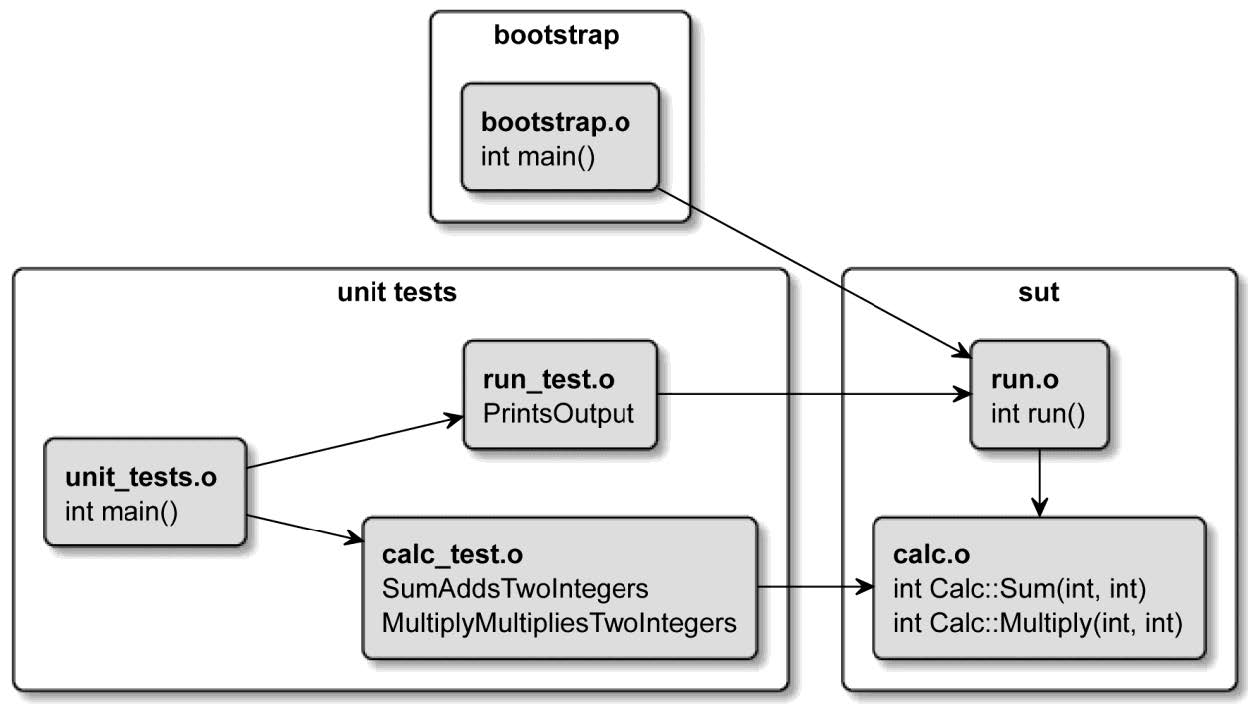
\includegraphics[width=0.8\textwidth]{content/3/chapter8/images/2.jpg}\\
图8.2 测试和生产可执行程序之间共享工件
\end{center}

最终得到了6个实现文件,它们将产生各自的(.o)目标文件:

\begin{itemize}
\item 
calc.cpp—要进行单元测试的Calc类。这称为被测单元(UUT),因为UUT是SUT的特化。

\item 
run.cpp—原来的入口点重命名为run(),现在可以对其进行测试。

\item 
bootstrap.cpp—新的main()入口点调用run()。

\item 
calc\_test.cpp—测试Calc类。

\item 
run\_test.cpp—run()的新测试可以放在这里。

\item 
unit\_tests.o—单元测试的入口点,扩展为run()的调用测试。
\end{itemize}

将要构建的库实际上不需要是一个实际的库:静态的或动态的。通过创建对象库,可以避免不必要的归档或链接。从技术上讲,通过依赖SUT的动态链接来节省一些时间是可能的,但我们在测试和SUT中都做了更改,抵消了潜在的收益。

来看看文件是如何改变的,从之前命名为main.cpp的文件开始:

\begin{lstlisting}[style=styleCXX]
// chapter08/02-structured/src/run.cpp

#include <iostream>
#include "calc.h"
using namespace std;

int run() {
	Calc c;
	cout << "2 + 2 = " << c.Sum(2, 2) << endl;
	cout << "3 * 3 = " << c.Multiply(3, 3) << endl;
	return 0;
}
\end{lstlisting} 

没有太多区别:重命名文件和函数。还添加了一个return语句,因为编译器不会对非main()的函数隐式执行此操作。

新的main()函数如下所示:

\begin{lstlisting}[style=styleCXX]
// chapter08/02-structured/src/bootstrap.cpp

int run(); // declaration
int main() {
	run();
}
\end{lstlisting} 

尽可能简单——声明链接器将从另一个翻译单元提供run()函数,并调用它。旁边的变化是src列表文件:

\begin{lstlisting}[style=styleCMake]
# chapter08/02-structured/src/CMakeLists.txt

add_library(sut STATIC calc.cpp run.cpp)
target_include_directories(sut PUBLIC .)

add_executable(bootstrap bootstrap.cpp)
target_link_libraries(bootstrap PRIVATE sut)
\end{lstlisting} 

首先,创建了一个sut库并进行标记。作为一个PUBLIC包含目录,这样将传播到所有将链接sut(即引导和单元\_tests)的目标。注意,include目录是相对于列表文件的,因此我们可以使用一个点(.)来引用当前的<source\_tree>/src目录。

是时候更新unit\_tests目标了。我们将删除对../src/calc.cpp文件的直接引用,并为unit\_tests目标添加到sut的链接引用。我们还将在run\_test.cpp文件中为主函数添加一个新的测试。为了简单起见,这里将跳过讨论,但若感兴趣,可以查看在线示例。同时,下面是整个测试列表文件:

\begin{lstlisting}[style=styleCMake]
# chapter08/02-structured/test/CMakeLists.txt

add_executable(unit_tests
				unit_tests.cpp
				calc_test.cpp
				run_test.cpp)
target_link_libraries(unit_tests PRIVATE sut)
\end{lstlisting} 

需要注册新的测试:

\begin{lstlisting}[style=styleCMake]
add_test(NAME SumAddsTwoInts COMMAND unit_tests 1)
add_test(NAME MultiplyMultipliesTwoInts COMMAND unit_tests 2)
add_test(NAME RunOutputsCorrectEquations COMMAND unit_tests 3)
\end{lstlisting} 

完成了!通过遵循此实践您可以确保在生产中使用的机器代码上执行测试。

\begin{tcolorbox}[colback=blue!5!white,colframe=blue!75!black,title=Note]
这里使用的目标名称sut和bootstrap,是为了从测试的角度非常清楚地说明它们的功能。实际项目中,应该选择与生产代码(而不是测试)的上下文相匹配的名称。例如,对于一个FooApp,命名你的目标foo而不是bootstrap, lib\_foo而不是sut。
\end{tcolorbox}

现在知道了如何在适当的目标中构建可测试项目,让我们将焦点转移到测试框架本身。我们不希望手动地将每个测试用例添加到列表文件中,对吧?
































